\documentclass[a4paper,10pt,oneside]{article}

\usepackage{graphicx}
\usepackage[top=1in,bottom=1in,left=1in,right=1in]{geometry}


\author{Luke Fraser}
\title{TMAker}
\date{\today}

\begin{document}
\section{Software}
The software design of the project consists of three central components segmentation, registration, and coring location positioning. Segmentation involves grouping the scanned biopsy images into separate regions as well as recognizing the cancerous region. The registration step maps the scanned biopsy image to an image of the current paraffin block ready for coring in the TMA machine. Defining a coring description is the step where each individual coring location is generated with respect to the paraffin block. With all 3 of these components in operation successful TMA's can be created.

\section{Image I/O}
The images acquired from the medical scanner were very large and they were compressed into two special formats, JPEG2000 and Aperio's Medical Imaging format. Each of the images were around 90,000x90,000 pixels. When compressed the images were around 300MB in size, but uncompressed would be around 15GB. This presented a challenge for processing images at such a large scale because they cannot be viewed in their entirety without filling the RAM of a modern computer. Also in many cases the full resolution was not needed or couldn't be used due to computational cost of processing so many pixels.

It was decided that using the original image formats was inconvenient. Both Aperio and JPEG2000 are not standard formats accepted by most image processing libraries making it difficult to read in data for processing. It was important to convert to a more standard format that could be used by both OpenCV and Matlab. First an attempt was made to directly convert from the Aperio format using the OpenSlide library directly into the TIFF format. This proved difficult to manage and it was taking up more time that it was worth considering the process would need to replicated for the JPEG2000 format as well. Learning all three image formats would have taken too long to understand in great detail. Other libraries were eventually used to make it easier to convert from the non-standard image formats.

The OpenTIFF format was used to process the images and store them in a tiled and pyramid image format. This allowed for different resolutions to be loaded without further processing and provided memory management by using the tiled image format. OpenTIFF is an open source library readily available on the Linux operating system making it convenient for this application. VIPS\cite[]<++> and Kakadu\cite[]<++> were the libraries used to convert the original image formats from the Aperio and JPEG2000 to OpenTIFF respectively. Once in the TIFF format it was much easier to load the images into RAM for processing. As well the TIFF format was directly supported by both Matlab and OpenCV making it much easier to load the images.

\section{Image Segmentation}
The scanned slide images prior to acquisition were stained providing color differences between cancerous and non-cancerous cells. At full resolution individual cell color contribution could be seen, but at lower resolutions the image appeared to have different color region descriptions. Where large concentrations of cancerous cells represented one color region and non cancerous cells represented another. This made color and obvious descriptor for segmentation.

The first segmentation attempt used histogram analysis to segment the pixels into regions. Each image was converted into the HSV(Hue Saturation and Value) color space. The Hue value could then be used because it is an unbiased descriptor of color in an image. A histogram of the Hue channel was created and the highest probable local maxima of the data set were accepted as the main color regions of the image. This naive approach however provided poor results and furthermore did not adequately segment the images. Although this method did provide useful segmentation information about the number of regions in the image.

The next approach involved using a K-means Squared segmentation to break up the image into cancerous and non-cancerous regions. Here the image was converted into the LAB color space. The LAB colorspace was used because pixels in the space are more evenly distributed across color and luminance. It is then easier to compare changes in luminance and color values against each other. It makes sense then that Euclidean distance between pixels in the LAB space provides better results than in a RGB space. The LAB image data was used for a 3-ways Kmeans segmentation. This limited the regions that kmeans sorted the pixels into to just 3 groups. The results from the Kmeans-squared segmentation were far superior to the previous histogram method. The kmeans was able to successfully segment between the cancerous and non-cancerous regions of the image with strong edges defined between the different regions. The resolution however was an important factor in both computation time as well as successful segmentation of every pixel in an image. As image size increased the Kmeans algorithm began to fail on every iteration resulting in unsuccessful segmentation.

The Kmeans segmentation was extended further by the work of the first histogram method. The histogram provided useful information on the number of regions in the image. To improve results from the histogram data filtering was used to smooth the histogram to provide better local maxima detection and remove spurious maxima. The local maxima thresholded below a probability and then counted to determine the number of regions present in the image. This value would then be sent to the kmeans algorithm to determine the proper regions for segmentation.

% limiting the pixel data
% deciding the desired number of regions
\section{Registration}
\begin{figure}[hbtp]
	\centering
	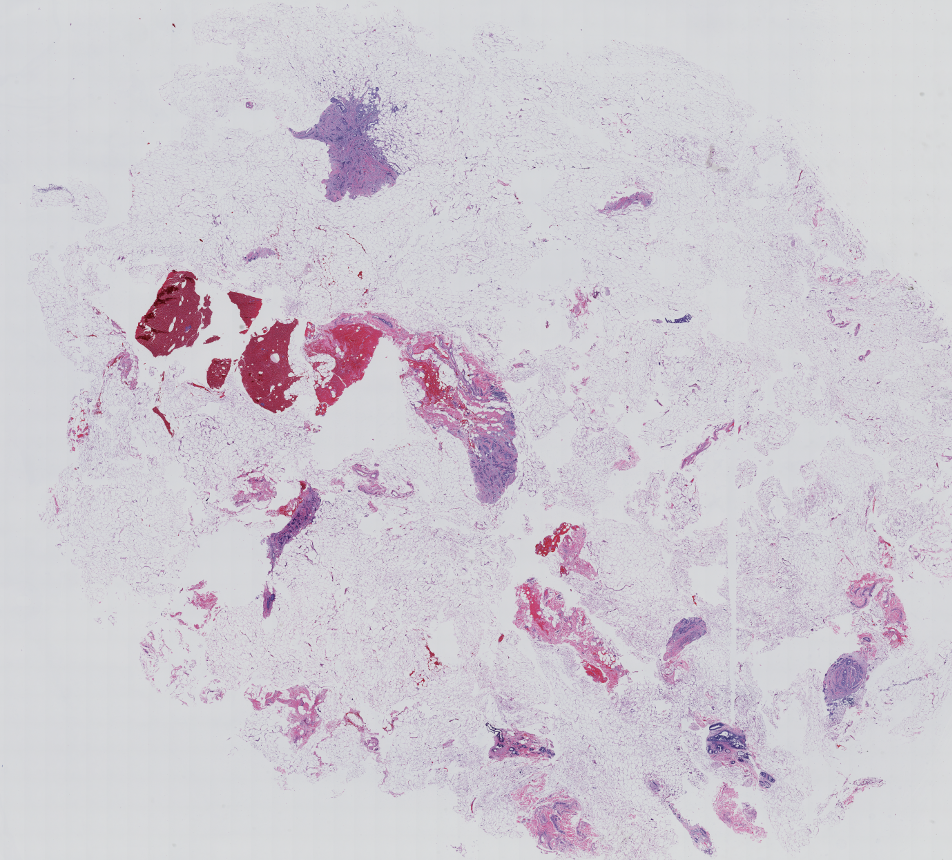
\includegraphics[height=3cm]{images/PO13-00516A1_1_7_201305171148.png}
	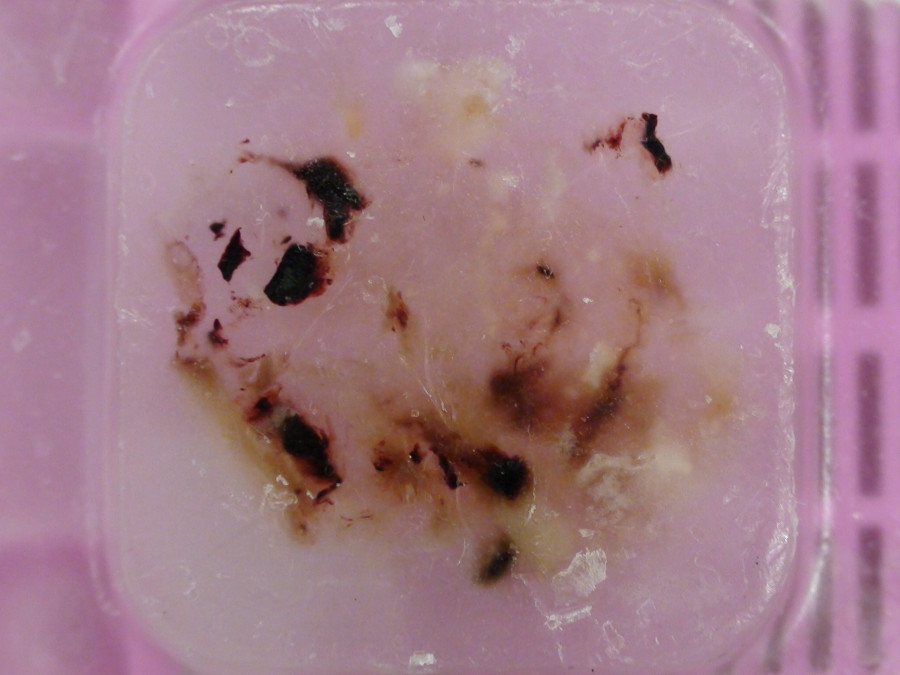
\includegraphics[height=3cm]{images/PO1300516_A1.JPG} 
	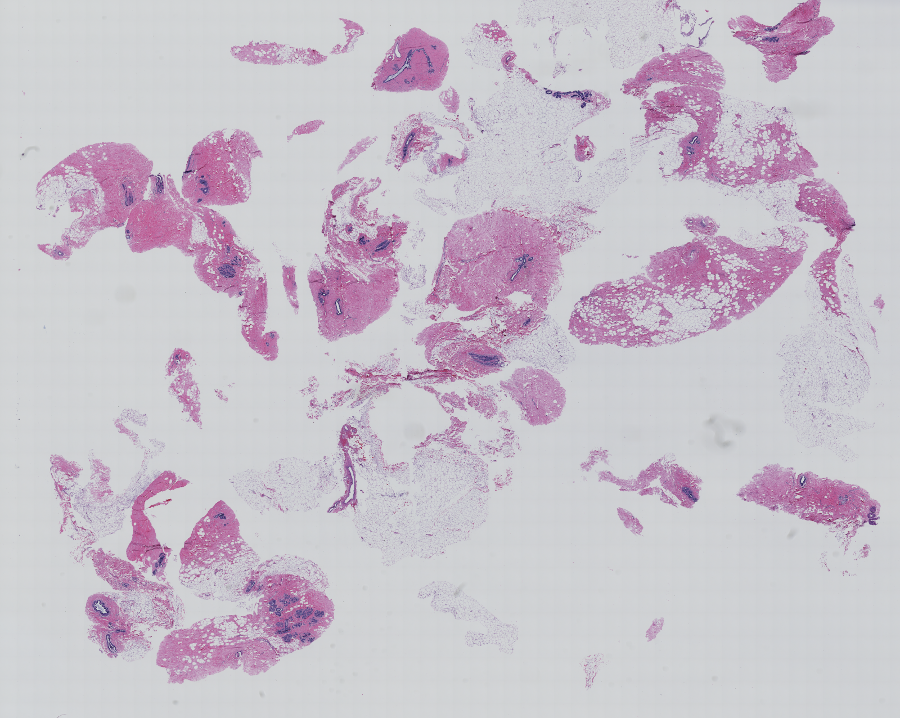
\includegraphics[height=3cm]{images/PO14-00496A1Level1_1_2_201404181459.png} 
	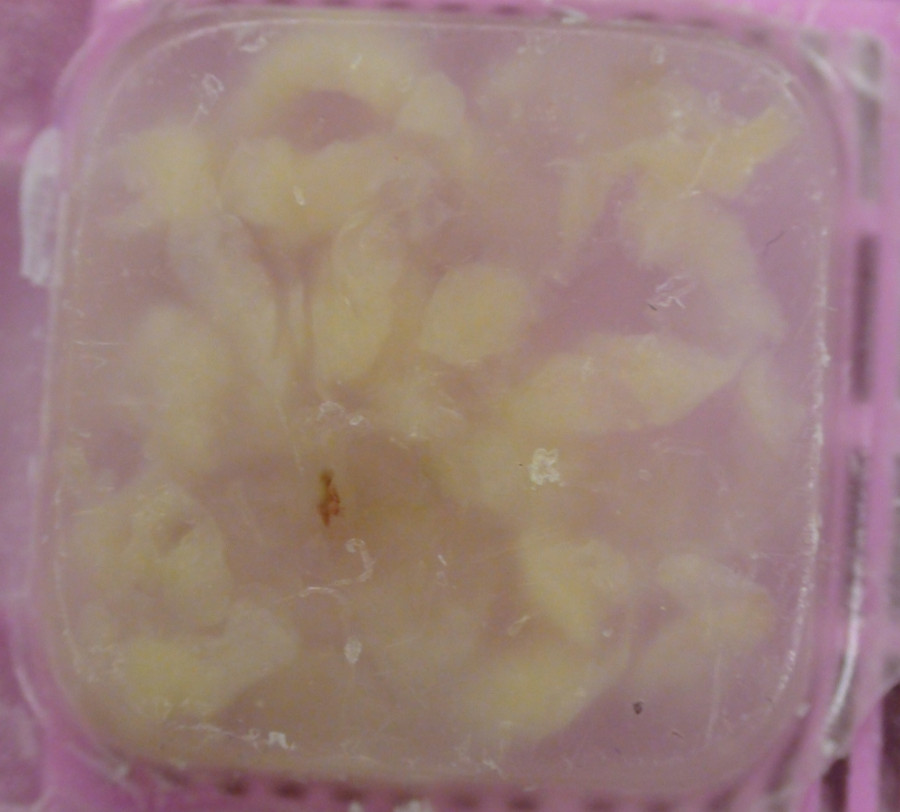
\includegraphics[height=3cm]{images/PO1400496_A1.JPG} 
	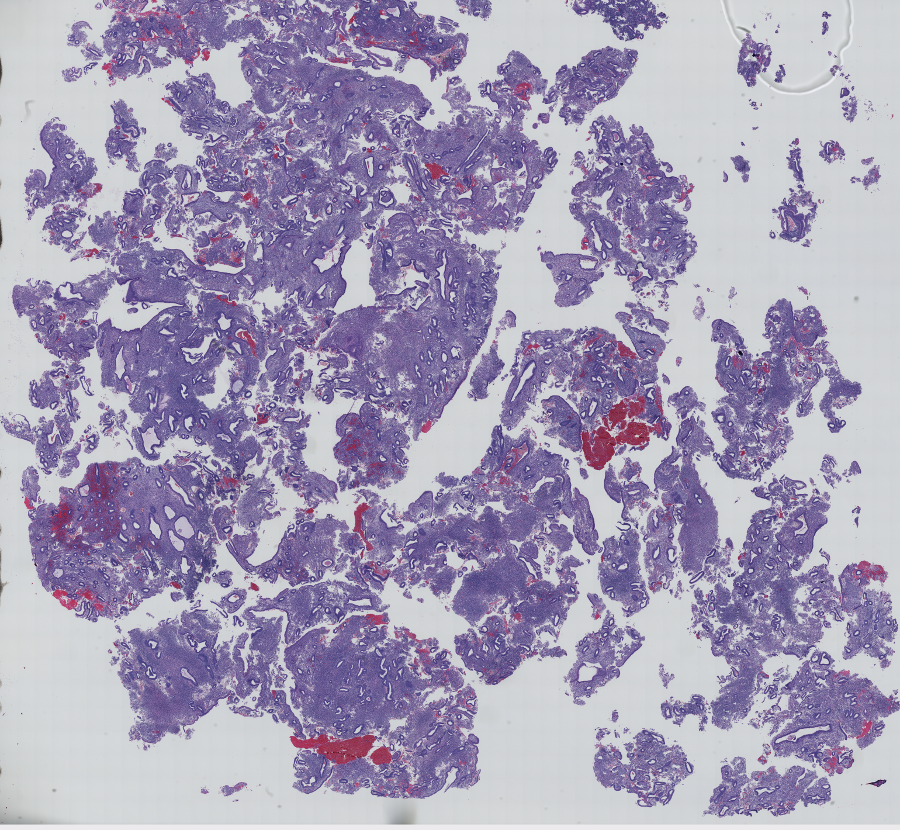
\includegraphics[height=3cm]{images/PO14-00482B3_1_2_201404171123.png} 
	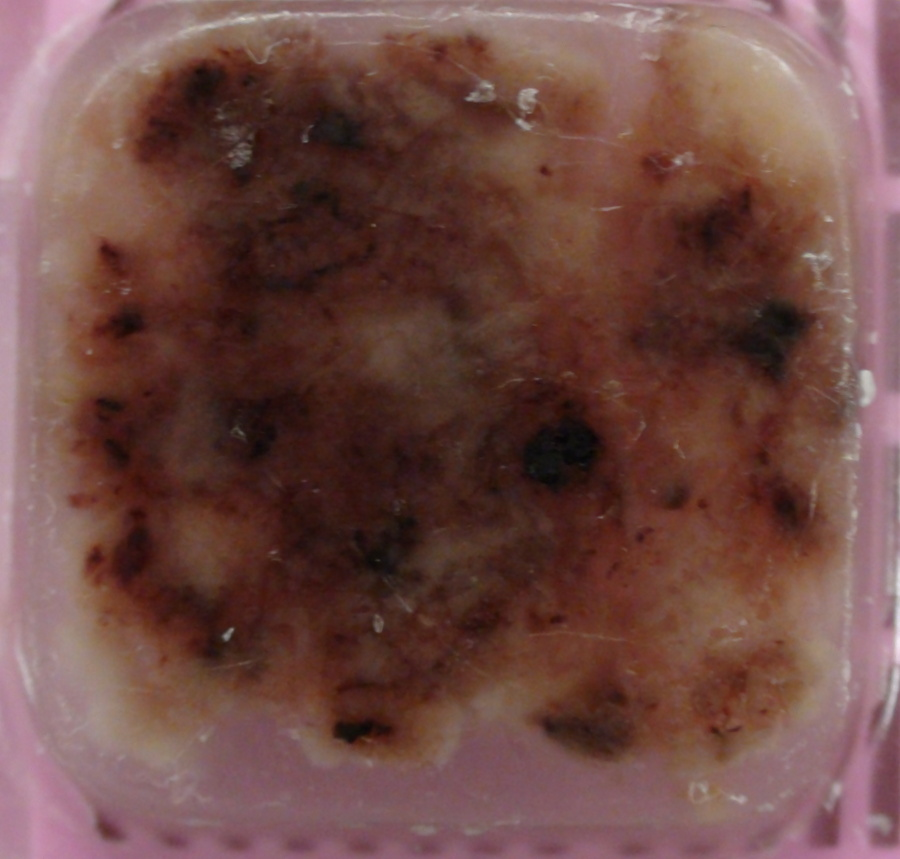
\includegraphics[height=3cm]{images/PO14004821_B3.JPG} 
	\caption{Image of subsurface tissue.}
	\label{fig:subsurface}
\end{figure}
Image registration is the step that allows to convert between the scanned image and the physical space of the paraffin block inside the mechanical TMA machine. Registration is central for coring the paraffin blocks without accurate registration the coring positions defined on the scanned image will not lineup with the paraffin block and the TMA will contain bad and unwanted tissue. The coring process proved to be a very difficult component. The two images that need to be registered are typically very different making it difficult for reliable registration. As seen in Figure the relation between the scanned image and the paraffin block image is limited. The lack of similarity is due to the fact that the scanned image is from a top layer slice of the paraffin block and does not contain subsurface tissue information that is present in the paraffin block image.
\end{document}
